\begin{figure*}[b!]
    \begin{subfigure}[c]{0.35\linewidth}
        \centering
        \begin{tikzpicture}[thick, scale=0.7, every label/.style={align=left, scale=0.7}]
            \pie[text=inside, sum=auto, color={blue!60, yellow!60, orange!60, red!60}]{
                19/,
                7/,
                6/,
                31/
            }
        \end{tikzpicture}
        \caption{Suggestions that should have been incorporated.}
        \label{fig:swebokUpdatesFull}
    \end{subfigure}
    \hfill
    \begin{subfigure}[c]{0.35\linewidth}
        \centering
        \begin{tikzpicture}[thick, scale=0.7, every label/.style={align=left, scale=0.7}]
            \pie[text=inside, sum=auto, color={blue!60, yellow!60, orange!60, red!60}]{
                19/,
                6/,
                6/,
                23/
            }
        \end{tikzpicture}
        \caption{Suggestions that may have been ignored intentionally.}
        \label{fig:swebokUpdatesCertain}
    \end{subfigure}
    \hfill
    \begin{subfigure}[c]{0.2\linewidth}
        \centering
        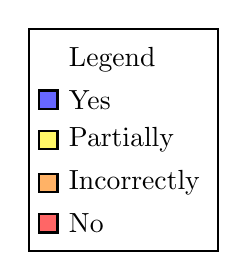
\begin{tikzpicture}
            \matrix [thick, draw=black] {
            \node[label=right:{Legend}] {}; \\
            \node[thick, shape=rectangle, draw=black, fill=blue!60,   label=right:{Yes}        ](0) {}; \\
            \node[thick, shape=rectangle, draw=black, fill=yellow!60, label=right:{Partially}  ](1) {}; \\
            \node[thick, shape=rectangle, draw=black, fill=orange!60, label=right:{Incorrectly}](2) {}; \\
            \node[thick, shape=rectangle, draw=black, fill=red!60,    label=right:{No}         ](3) {}; \\
            };
        \end{tikzpicture}
    \end{subfigure}
    \caption{Breakdown of how many suggestions we made on the \acs{swebok} V4
        \citep{SWEBOK2024} were incorporated into the final version
        \citeyearpar{SWEBOK2025}.}\label{fig:swebokUpdates}
\end{figure*}
